% 6) Surgimiento de la computación cuantica por parte de IBM y Qiskit
En el área de la matemáticas, la factorización es una técnica que consiste en la descomposición en factores de una expresión algebraica
en forma de un producto. El teorema fundamental de la aritmética cubre la factorización de números enteros, este teorema pertenece a la teoría
de números. El teorema de factorización afirma lo siguiente:
\begin{teor}
    Cada entero positivo tiene una única descomposición en números primos.
    \label{teo:enterosprimos}
\end{teor}
El teorema fue demostrado por primera vez por Euclides, aunque la primer demostración completa apareció en las \textit{Disquisitiones Arithmeticae}
de Carl Friedrich Gauss.\\
El análisis numérico es el estudio de algoritmos, el cual consiste en un conjunto de instrucciones o reglas ordenadas y finitas que permiten
realizar una actividad mediante pasos sucesivos con el proposito de resolver problemas matemáticos dentro de la matemática continua, esto da 
una aproximación numérica. Hay problemas sencillos de calcular como una raiz cuadrada, no tienen soluciones exactas o son costosas en tiempo
para obtenerlas.Para obtener una aproximación útil, se debe conocer la presición de los resultados y cuantos recursos se necesita para lograrlo, estos conceptos
cuantificados son conocidos como \textit{presición, convergencia, estabilidad y complejidad.}\\\\
La complejidad algorítmica, informalmente, es una medida que permite a los programadores conocer la cantidad de recursos que necesita un algoritmo para resolver un problema en función de su tamaño. El objetivo es
comparar la eficiencia de algoritmos a la hora de resolver un problema conocido\cite{Cohen1998}. Para realizar una clasificación en la complejidad de un algoritmo
se usa normalmente la notación asintótica, la cual es que por el número de operaciones básicas ejecutadas por un algirtmo se obtiene una función. Cada
una se ve denotada por $T(N)$, donde $N$ es el número de elementos numéricos dentro del algoritmo. Para valores pequeños de N, las constantes 
que acompañan a los términos de la función $T$ pueden influir de manera significativa al coste tota y con ello obtener conclusiones erroneas respecto
a la eficiencia del algoritmo. En cambio este tipo de análisis se realiza con números grandes de $N$. Deendiendo del análisis que se realice, podemos
encontrar diferentes tipos de notaciones. La notación más usada es la llamada O grande y se denota por $O$.
\begin{defi}
Se dice que un algoritmo F tiene una complejidad $O(G(N))$ si existen dos constantes $C$ y $N_0$ para las que se cumpla $|F(N)|<C\cdot G(N)$ para todo
$N>N_0$
\end{defi}
En otras palabras, que el algoritmo F tiene una complejidad $O(G)$ si el número de operaciones necesarias es constante para un número grande de N. Un ejemplo
de esta clasificación puede observarse en la siguiente tabla: algorit
\begin{table}[H]
    \centering
    \begin{tabular}{lll}
        \hline
        Notación & Nombre & Ejemplo de algoritmo \\
        \hline
        $O(1)$ & Constante & Acceso a un elemento de un vector\\ 
        $O(log N)$ & Logarítmica& Búsqueda binaria\\
        $O(N)$ & Lineal & Búsqueda secuencial\\
        $O(N log N)$ & Lineal-Logarítmica& Algoritmo de ordenamiento \textit{quicksort}\\
        $O(N^2)$ &Cuadrática & Algoritmo de ordenamiento simple\\
        $O(N^3)$ &Cúbica & Multiplicación de matrices\\
        $O(2^N)$ &Exponencial & Partición de conjuntos\\ \hline
    \end{tabular}
    \caption{Ejemplos de algoritmos numéricos con su clasificación $O$ de complejidad}
    \label{tabla:notacion-O}
\end{table}
La mayor parte de los algoritmos de factorización elementales son de proposito general, es decir, permiten descomponer cualquier
número introducido, la diferencia entre algoritmos es el tiempo que se toman para encontrar la factorización del número dado. El problema de 
factorizar enteros de tiempo polinómico no ha sido resulto en computación clásica. Esto puede ser de gran ayuda al avance en el ambito de la 
criptografía, ya que muchos sistemas criptográficos dependen de la imposibilidad de ser resueltos en un tiempo corto. La complejidad de este problema se encuentra en el núcleo de varios sistemas criptográficos importantes. Un algoritmo veloz para la factorización
de enteros significaría que el algoritmo de clave pública RSA es inseguro. Si un número grande, de $b$ bits es el producto de dos primos
de aproximadamente el mismo tamaño, no existe algoritmo conocido capaz de factorizarlo en tiempo polinómico. Esto significa que ningún algoritmo
conocido puede factorizarlo en tiempo O$(b^K)$, para cualquier constante $k$. Aunque, existen algoritmos que son más rápidos que O$(a^b)$ para cualquier a 
mayor que 1. En otras palabras, los mejores algoritmos son súper-polinomiales, pero sub-exponenciales. En particular, el mejor tiempo
asintótico de ejecución lo contiene el algoritmo de \textit{criba general del cuerpo de números\cite{Agrios2003} (CGCN)}, que para un número n es:
\begin{equation}
    O\left(exp\left(\left(c+\epsilon_n\right) \left(\ln p\right)^\frac{1}{3} \left(\ln(\ln p)\right)^\frac{2}{3} \right) \right).
    \label{eq:O(clasico)}
\end{equation}
Para una computadora ordinaria, la CGCN es el mejor algoritmo conocido para números grandes.\\
Al inicio de la decada de 1960, Rolf Landauer se cuestionaba acerca de si las leyes físicas determinaban limites a los procesos de computo. En concreto
se interesó por el origen del calor disipado por los ordenadores. Uno de los problemas actuales de los ordenadores de alta velocidad
es el calor que se produce durante su funcionamiento. Cada vez se fabrican más microchips más pequeños en el cual se administra una mayor cantidad de transistores, sin embargo, 
existe un límite en el cual podemos ir disminuyendo el tamaño de cada transistor debido a que los canales donde circulan los electrones pueden escaparse por el fenómeno del 
efecto tunel, es por ello que la computación digital clásica no debe estar muy lejos del límite.\\\\

Las ideas esenciales de la computación cuántica surgieron en los primeros años de la decada 1980, esto de la mente de Paul Beinoff, quien hacia operar computadoras clásicas
con operaciones cuánticas. Entre 1981 y 1982, Richard Feymann propusó el uso de fenónemos cuánticos para realizar cálculos computacionales exponiendo la idea que, dada la naturaleza
de la mecánica cuántica algunos procesos se realizarian en un menor periodo de tiempo a comparación de una computadora clásica. En 1985, David Deutsch describió el primer computador cuántico
universal, este ordenador era capaz de simular cualquier otro computador cuántico por medio de la tesis de Church-Turing ampliado, el cual es un enunciado formalmente indemostrable, no obstante, tiene una aceptación
universal. Las tesis de Church y Turing son las siguientes:
\begin{tesis}[de Church]
    La clase de las funciones que pueden ser calculadas mediante un algoritmo coincide con la clase de las funciones recursivas.
\end{tesis}
\begin{tesis}[de Turing]
    La clase de las funciones que pueden ser calculadas mediante un método definido coincide con la clase de las funciones calculables mediante una Máquina de Turing.
\end{tesis}
En base a estos enunciados, surgió la idea de que un computador cuántico podría ejecutar diferentes algoritmos cuánticos. A lo largo de la decada de 1990, la teoría acerca de la computación
cuántica empezó a tener sus primeras aplicaciones en forma de algoritmos cuánticos, el primero en realizar estos aportes Dan Simon demostrando la ventaja de usar un computador cuántico frente a uno tradicional
al comparar el modelo de probabilidad clásica con el modelo cuántico. Sus ideas sirvieron como base para el desarrollo de algoritmos de auténtico interés práctico. En el año 1993, Charles Benett descubre 
el tele-transporte cuántico, que abre una nueva vía de investigación dirigida hasta las comunicaciones.\\
Entre 1994 y 1995 Peter Shor definió el algortimo que permite calcular los factores primos de números a un tiempo menor a cualquier computadora clásica. En el año 2000, IBM diseña un computador cuántico de 5 qubits capaz de 
ejecutar un algoritmo de búsqueda de orden que forma parte del algoritmo de Shor. El algoritmo de Shor tiene una complejidad algorítmica \cite{Shor1997}
\begin{equation}
    O(logN)^3.
\end{equation}
 En 2001, nuevamente, IBM en conjunto con la Universidad de 
Standford, consiguen ejecutar por primera vez el algoritmo de Shor en el primer computador cuántico de 7-qubits, en el experimento se calcularon los factores primos de 15, dando como resultado 3 y 5 utilizando para ello 1018 moléculas, cada una de ellas con 7 átomos.\\\\
\begin{figure}[H]
    \begin{subfigure}{0.5\textwidth}
        \centering
        \caption{}
    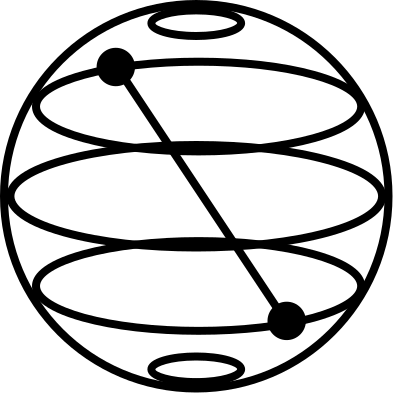
\includegraphics[height=5cm]{images/Qiskit.png}
    \label{fig:logo_qiskit}
    \end{subfigure}
    \begin{subfigure}{0.5\textwidth}
        \centering
        \caption{}
    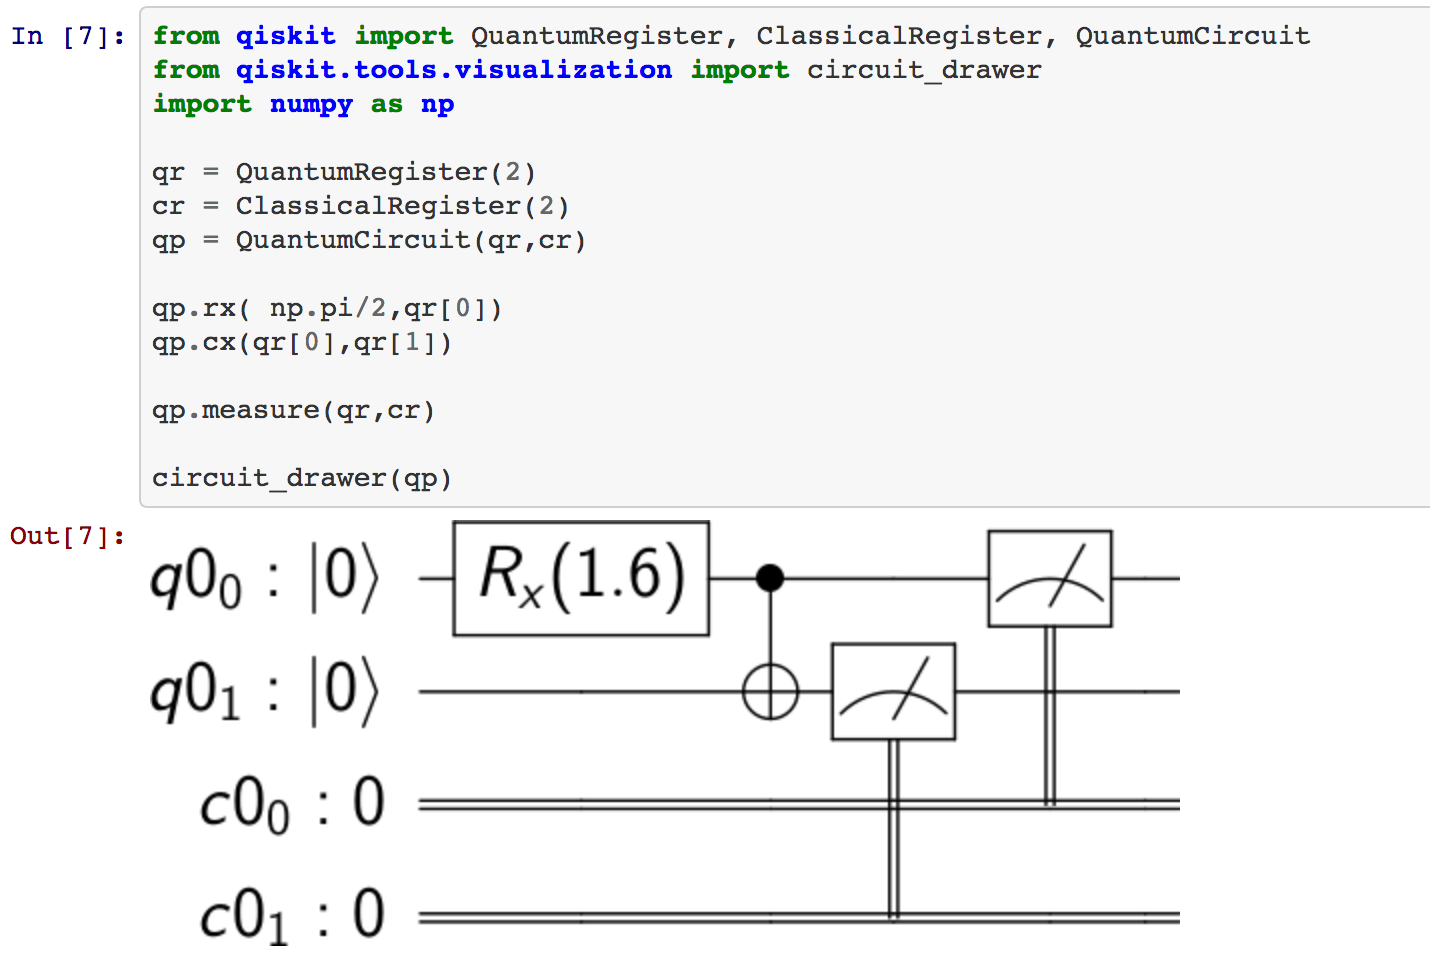
\includegraphics[height=5cm]{images/Example_qiskit.png}
    \label{fig:example_qiskit}
    \end{subfigure}
    \caption{(a) Logo de Qiskitl, (b) Ejemplo de un circuito cuántico implementado dentro de Jupyter Notebook de Python.}
\end{figure}
En el año 2017, IBM lanzo su primer version de la libreria \href{https://qiskit.org/}{Qiskit}, la cual, es un framework de libre acceso para computación cuántica. El framework te provee de herramientas para la creación y manipulación de programas cuánticos
y correrlos en los prototipos de dispositivos cuánticos llamados \href{https://quantum-computing.ibm.com/}{\textit{IBM Q Experience}}. Este framework esta desarrollado en el lenguaje \textit{Python}. 